\documentclass[10pt, a4paper]{report}
\usepackage[utf8]{inputenc}
\usepackage{booktabs}
\usepackage{multirow}
\usepackage[table,xcdraw]{xcolor}
\usepackage{adjustbox,lipsum}
\usepackage{csquotes}
\usepackage{graphicx}
\newcommand{\myparagraph}[1]{\paragraph{#1}\mbox{}\\} %used for better formating of some text

\setlength{\oddsidemargin}{0cm}
\setlength{\evensidemargin}{0cm}
\setlength{\textwidth}{500pt}

\title{Report on Certificate Tools}
\author{Oliver Bodnár}
\date{August 2016}

\begin{document}

\maketitle

\tableofcontents

\newpage

\part{Overview}

\chapter{Overview Tables}

\section{General}
%TABLE START
\begin{table}[h!]
\centering
\caption{Overwiew General}
\label{my-label}
\begin{adjustbox}{max width=\textwidth}
\begin{tabular}{|c|c|c|c|c|}
\hline
                        & \multicolumn{4}{c|}{General}                                                                               \\ \cline{2-5} 
\multirow{-2}{*}{Tools} & Type   & View + info                                        & License & Operating System                   \\ \hline
OpenSSL                 & PKCS12 & \cellcolor[HTML]{34FF34}Yes                        & Public  & \cellcolor[HTML]{34FF34}Both       \\ \hline
Keytool                 & JKS    & \cellcolor[HTML]{34FF34}{\color[HTML]{000000} Yes} & Public  & \cellcolor[HTML]{34FF34}Both       \\ \hline
GnuPG                   &        &                                                    &         &                                    \\ \hline
Keystore Explorer       & Both   & \cellcolor[HTML]{34FF34}Yes                        & Public  & \cellcolor[HTML]{FFC702}Win | OS X \\ \hline
\end{tabular}
\end{adjustbox}
\end{table}
%TABLE END

\subsection{Type}
This section defines type of storage file in which the certificates or keys are saved. Most common are PKCS\#12 (.pfx and .p12 extentions) and JKS (Java KeyStore). 

\subsection{View and information}
This section shows whether it is possible to view certificates or keys and additional information. Yes means that at least viewing is supported while not necessary meaning possibility of viewing more information about certificate.

\subsection{License}
Type of license and possibility of using said tool for testing or production code. Public means that license is not requiered for use in production code but does not mean that it should be used as such. Definition if it is advised to use said tool in production code or only in testing enviroment will be talked about in the next chapter under each tool.

\subsection{Operating Systems}
In this part the Operating System where the tool is imported is defined. Both means that it is implemented under UNIX like systems and Windows systems. Otherwise the Operating System is defined (Windows | UNIX).

\newpage

\section{Generation and signing of certificates}

\subsection{Keys, certificates and basic constraints}
%TABLE START
\begin{table}[h!]
\centering
\caption{Generation of keys and certificates and basic constrints}
\begin{adjustbox}{max width=\textwidth}
\begin{tabular}{|c|c|c|c|c|c|c|}
\hline
                       & \multicolumn{4}{c|}{Generate keys}                                                                                                                             & \multicolumn{2}{c|}{Basic Constraints}                    \\ \cline{2-7} 
\multirow{-2}{*}{Tool} & \begin{tabular}[c]{@{}c@{}}+\\  self-signed certificate\end{tabular} & + CSR                       & Specify length              & Specify algorithm           & Specify Type                & Specify path length         \\ \hline
OpenSSL                & \cellcolor[HTML]{34FF34}Yes                                          & \cellcolor[HTML]{34FF34}Yes & \cellcolor[HTML]{34FF34}Yes & \cellcolor[HTML]{34FF34}Yes & \cellcolor[HTML]{34FF34}Yes & \cellcolor[HTML]{34FF34}Yes \\ \hline
Keytool                & \cellcolor[HTML]{34FF34}Yes                                          & \cellcolor[HTML]{34FF34}Yes & \cellcolor[HTML]{34FF34}Yes & \cellcolor[HTML]{34FF34}Yes & \cellcolor[HTML]{34FF34}Yes & \cellcolor[HTML]{34FF34}Yes \\ \hline
GnuPG                  &                                                                      &                             &                             &                             &                             &                             \\ \hline
Keystore explorer      & \cellcolor[HTML]{34FF34}Yes                                          & \cellcolor[HTML]{34FF34}Yes & \cellcolor[HTML]{34FF34}Yes & \cellcolor[HTML]{34FF34}Yes & \cellcolor[HTML]{34FF34}Yes & \cellcolor[HTML]{34FF34}Yes \\ \hline
\end{tabular}
\end{adjustbox}
\end{table}
%TABLE END

\subsubsection{Generate keys}

\paragraph{Self-signed certificate}
possibility of using 1 command to generate key pair and self-signed certificate

\paragraph{Certificate Signing Request}
possibility of using a command to generate key pair and certificate signing request to certificate authority.

\paragraph{Specify length}
possibility to specify the length of output key

\paragraph{Specify algorithm}
possibility to choose between different types of algorithms for key generation


\subsubsection{Basic Constraints}

\paragraph{Specify Type}
specify if generated certificate will belong to certificate authority or whether it will be end certificate

\paragraph{Specify path length}
specify the maximum length of certificate authority chain


\subsection{Specifications}

%TABLE START
\begin{table}[h!]
\centering
\caption{Specifications}
\label{my-label}
\begin{adjustbox}{max width=\textwidth}
\begin{tabular}{|c|c|c|c|c|c|}
\hline
                       &                               &                                          &                                                &                                            &                                                                             \\
\multirow{-2}{*}{Tool} & \multirow{-2}{*}{CSR signing} & \multirow{-2}{*}{Privkey + signed chain} & \multirow{-2}{*}{Specify certificate validity} & \multirow{-2}{*}{SAN for end certificates} & \multirow{-2}{*}{\begin{tabular}[c]{@{}c@{}}Support for\\ CSP\end{tabular}} \\ \hline
OpenSSL                & \cellcolor[HTML]{34FF34}Yes   & \cellcolor[HTML]{34FF34}Yes              & \cellcolor[HTML]{34FF34}Yes                    & \cellcolor[HTML]{34FF34}Yes                & \cellcolor[HTML]{34FF34}Yes                                                 \\ \hline
Keytool                & \cellcolor[HTML]{34FF34}Yes   & \cellcolor[HTML]{34FF34}Yes              & \cellcolor[HTML]{34FF34}Yes                    & \cellcolor[HTML]{34FF34}Yes                & \cellcolor[HTML]{34FF34}Yes                                                 \\ \hline
GnuPG                  &                               &                                          &                                                &                                            &                                                                             \\ \hline
Keystore explorer      & \cellcolor[HTML]{34FF34}Yes   & \cellcolor[HTML]{34FF34}Yes              & \cellcolor[HTML]{34FF34}Yes                    & \cellcolor[HTML]{34FF34}Yes                & \cellcolor[HTML]{FE0000}No                                                  \\ \hline
\end{tabular}
\end{adjustbox}
\end{table}
%TABLE END

\paragraph{Certificate Signing Request signing}
possibility of signing a certificate signing request with certificate authority's key

\paragraph{Create combination of private key and signed chain}
possibility of generating private key and chain signed by certificate authority that will be outputed to a single file

\paragraph{Specify certificate validity}
possibility of choosing how long will the certificate be valid. This should be done by certificate authority.

\paragraph{Setting Subject Alternative Name for end certificates}
possibility of choosing Subject Alternative Name for end certificates. That should be done by IP's or DNS addresses.

\paragraph{Support for Cryptographic Service Provider}
whether the use, choosing and changing of Cryptographic Service Provider is supported.


\section{Conversions}

%TABLE START
\begin{table}[h!]
\centering
\caption{Conversions}
\label{my-label}
\begin{adjustbox}{max width=\textwidth}
\begin{tabular}{|c|c|c|c|c|}
\hline
                        & \multicolumn{4}{c|}{Conversions}                                                                                                                                            \\ \cline{2-5} 
                        & \multicolumn{2}{c|}{Exporting}                                 &                                         &                                                                  \\ \cline{2-3}
\multirow{-3}{*}{Tools} & Certificate/chain only from file & Private key only            & \multirow{-2}{*}{Direct JKS and PKCS12} & \multirow{-2}{*}{Import certificate and private key into a file} \\ \hline
OpenSSL                 & \cellcolor[HTML]{34FF34}Yes      & \cellcolor[HTML]{34FF34}Yes & \cellcolor[HTML]{FF3A3A}No              & \cellcolor[HTML]{34FF34}Yes                                      \\ \hline
Keygen                  & \cellcolor[HTML]{34FF34}Yes      & \cellcolor[HTML]{FE0000}No  & \cellcolor[HTML]{34FF34}Yes             & \cellcolor[HTML]{34FF34}Yes                                      \\ \hline
GnuPG                   &                                  &                             &                                         &                                                                  \\ \hline
Keystore explorer       & \cellcolor[HTML]{34FF34}Yes      & \cellcolor[HTML]{34FF34}Yes & \cellcolor[HTML]{34FF34}Yes             & \cellcolor[HTML]{34FF34}Yes                                      \\ \hline
\end{tabular}
\end{adjustbox}
\end{table}
%TABLE END


\subsection{Exporting}

\subsubsection{Certificate or certificate chain from a file}
Possibility of extracting certificate or certificate only from a file. Choice of Yes based on possibility of extracting either from a file.

\subsubsection{Private key only}
Possibility of extracting private key from tool's file storage type of choice.

\subsection{Direct conversion between Java Keystore and PKCS\#12 file}
Possibility of direct conversion (by a command of tested tool) between Java KeyStore and PKCS\#12 type file.

\subsection{Importing of certificates and keys into storage files}
Possibility of importing (additional?) certificates and keys into storage files of said tool. Yes if it is possible to import or add another certificate or key into storage.


\newpage
%TOOLS PART
\part{Tools}

%OPENSSL text added by parts, need to check commands again
\chapter{OpenSSL}

\section{General}

  \subsection{Type}
  OpenSSL uses PKCS12 to store keys and or certificates. Certificates and keys  made in OpenSSL however are being made into PEM or DER encoded file. Said keys/certificates can then be stored inside single .pfx file. 
  
  \subsection{View and information}
  
\subsubsection{Viewing stored certificates}
\myparagraph{PEM encoded certificates (.pem$\vert$.cer$\vert$.crt):}
  \begin{verbatim}
  openssl x509 -in sample_cert.extention -text -noout
  \end{verbatim}
\myparagraph{DER encoded certificates (.der):}
  \begin{verbatim}
  openssl x509 -in certificate.der -inform der -text -noout
  \end{verbatim}
\myparagraph{Importing PEM or DER encoded keys or certificates into PKCS\#12 file:}
  \begin{verbatim}
  openssl pkcs12 -export -in file.pem \
          -inkey privateKeyFile.key -out file.p12 \
          -name "My Certificate" -certfile othercerts.pem
  \end{verbatim}
certfile option is used only if importing more certificates into a single PKCS\#12 file is wanted.

  
  \subsection{License}
OpenSSL is free to use commercialy, however creating CA is not advised in O'REILLY's Network Security with OpenSSL by J. Viega, M. Messier and P. Chandra on page 59,
\begin{displayquote}
Since OpenSSL's command-line CA functionality was intended primarely as an example of how to use OpenSSL to build a CA, we don't recommend that you attempt to use it in a large production environment.
\end{displayquote}
and also hinted in manual pages:
\begin{displayquote}
The ca command is quirky and at times downright unfriendly.

The ca utility was originally meant as an example of how to do things in a CA . It was not supposed to be used as a full blown CA itself: nevertheless some people are using it for this purpose.

The ca command is effectively a single user command: no locking is done on the various files and attempts to run more than one ca command on the same database can have unpredictable results. 
\end{displayquote}
  
\section{Generation and signing of certificates}

  \subsection{Keys, certificates and basic constraints}
  
    \subsubsection{Generate keys}
    
      \paragraph{Self-signed certificate}
      It is possible to generate private key and self signed certificate with 
      \begin{verbatim}
      openssl req -x509 -sha256 -nodes -days 365 \
	      -newkey rsa:[length] -keyout privateKey.key \
              -out certificate_name.crt
      \end{verbatim}
      
      \paragraph{Certificate Signing Request}
      It is possible to generate private key and CSR with
      \begin{verbatim}
      openssl req -out CSR.csr -new -newkey rsa:[length] \
              -nodes -keyout privateKey.key
      \end{verbatim}
      
      \paragraph{Specify length}
      Length is specified while generating key/certificate.
      
      \paragraph{Specify algorithm}
      Currently OpenSSL supports Public-key cryptography algorithms:
      RSA, DSA, Diffie-Hellman key exchange, Elliptic Curve
      
      In the past also support for GOST R 34.10-2001 but as of January 2016 deprecated (https://mta.openssl.org/pipermail/openssl-commits/2016-January/003023.html )
      
      
    \subsubsection{Basic constraints}
    
    Basic constraints are defined in CA's openssl.cnf \verb+[ v3_req ]+ part.
    \begin{verbatim}
[ v3_req ]

basicConstraints=critical,CA:<BOOL_VAL>, pathlen:<maxChainLengthInteger>
    \end{verbatim}

      \paragraph{Specify Type}
To specify if generated certificate belongs to CA or is end certificate you choose \verb+<BOOL_VAL>+ true or false respectively.
      \paragraph{Specify path length}
Specifying of path length is made by setting a \verb+<maxCheinLengthInteger>+ to desired value (e.g. if generated certificate should be used only for generating end certificates the value is 0)
  \subsection{Specifications}
  
    \subsubsection{Certificate Signing Request signing}
   SR signing can be done by CA created in openSSL by command
\begin{verbatim}
openssl ca -config ca/openssl.cnf \
        -extensions server_cert -days <validity_time>  \
	-notext -md [message digest alg] -in ca/csr/www.example.com.csr.pem \
        -out ca/certs/www.example.com.cert.pem
\end{verbatim}

    \subsubsection{Create combination of private key and signed chain}
    First creation of the request is needed, after that request must be signed. To combine them together the creation of PKCS\#12 file is needed with commands:
\begin{verbatim}
	openssl pkcs12 -export -out outfilename.p12 \
	        -in signed_certificate.crt -inkey privateKey.key \
	        -chain -CAfile ca-all.crt -password pass:PASSWORD
\end{verbatim}
    \subsubsection{Specify certificate validity}
    Time how long the certificate will be valid can be given in csr but only as a suggestion. Ultimately the real time of validity is always given by CA signing the CSR.
    \subsubsection{Setting Subject Alternative Name for end certificates}
    The Subject Alternative Name is also given in \verb+[ v3_req ]+ part of openssl.cnf that CA uses. It can be given as an IP address but also as a DNS name.

\begin{verbatim}
[ v3_req ]
subjectAltName = @alt_names

[alt_names]
DNS.1 = example1.com
DNS.2 = example2.com
DNS.<next_number> = dns_webaddress.com
\end{verbatim}

    \subsubsection{Support for Cryptographic Service Provider}
OpenSSL has native support for Cryptographic Service Provider since version 0.9.7 by creating PKCS\#12 file using -CSP option to set the cspname parameter

%Not totally sure of this http://www.drh-consultancy.demon.co.uk/pkcs12faq.html is my refference
    
\section{Conversions}

  \subsection{Exporting}
  
    \subsubsection{Certificate or certificate chain from a file}
    To export certificate from a PKCS\#12 file use:
\begin{verbatim}
openssl pkcs12 -in name.[pfx|p12] -nokeys -clcerts -out name.pem
\end{verbatim}

    To export certificate chain from a PKCS\#12 file use:
\begin{verbatim}
openssl pkcs12 -in name.[pfx|p12] -nokeys -cacerts -out CAchain.pem
\end{verbatim}
    It should be mentioned that if there are multiple certificates in a chain they are all going to be in same output file.

    \subsubsection{Private key only}
    To export an encrypted private key use:
\begin{verbatim}
openssl pkcs12 -in name.[pfx|p12] -nocerts -out name.encrypted.priv.key
\end{verbatim}

    To export an unencrypted private key use:
\begin{verbatim}
openssl pkcs12 -in name.[pfx|p12] -nocerts -nodes -out name.unencrypted.priv.key
\end{verbatim}


  \subsection{Direct conversion between Java Keystore and PKCS\#12 file}
Direct conversion between Java Keystore and PKCS\#12 type file is not supported by OpenSSL 
  \subsection{Importing certificates and keys into storage files}
To import certificate and private key into a single PKCS\#12 type file use:
\begin{verbatim}
 openssl pkcs12 -export -out certificate.pfx \
         -inkey privateKey.key -in certificate.crt \
         -certfile CACert.crt
\end{verbatim}


\chapter{Keytool}

\section{General}

  \subsection{Type}
Keytool has native support for both PKCS\#12 and Java KeyStore type files 
  \subsection{View and information}
To view information about PEM or DER encoded certificate use:
\begin{verbatim}
keytool -printcert -file certificate.extention
\end{verbatim}

To view information about Jave KeyStore or PKCS\#12 encoded file use:
\begin{verbatim}
keytool -list -v -keystore store_file.[pfx|p12|jks]
\end{verbatim}

Viewing Public key part of certificate is not availiable in keytool.
  \subsection{License}
Keytool is free to use in production code and is licensed under Apache Licence Version 2.0. For more detailed description look at http://www.apache.org/licenses/LICENSE-2.0.txt
  
\section{Generation and signing of certificates}

  \subsection{Keys, certificates and basic constraints}
  
    \subsubsection{Generate keys}
    
      \paragraph{Self-signed certificate}
To generate new key pair and self-signed certificate use:
\begin{verbatim}
keytool -genkey -keyalg [RSA|DSA] -alias [alisaname] \
        -keystore [keystore_file] -storepass [password] \
        -validity [time] -keysize [length]
\end{verbatim}

Keytool natively supports only DSA of length in between 512 and 1024, and is considered to be dangerous to use. RSA with key length of at least 2048 is preffered.

      \paragraph{Certificate Signing Request}
To generate a Certificate Signing Request generation of a key pair with alias is needed:
\begin{verbatim}
keytool -genkey -alias namealias -keyalg [RSA|DSA] \
        -keysize [length] -keystore [keystore_path | new_keystore_name]
\end{verbatim}
To create a CSR you then need to do:
\begin{verbatim}
keytool -certreq -keyalg [keyalg_from_genkey] -alias [alias_from_genkey] \
        -file certreq.csr -keystore [jks_from_genkey]
\end{verbatim}
Where you need to set -keyalg -alias and -keystore as chosen when generating key pair earlier.

      \paragraph{Specify length}
Length is specified when generating keys, RSA support for up to 4096, DSA support from 512 up to 1024.

      \paragraph{Specify algorithm}
Algorithm is specified while generating key pair, currently support for DSA, RSA. EC is needed to be implemented.      
    \subsubsection{Basic constraints}
    
      \paragraph{Specify Type}
With keytool you can make a self-signed CA certificate by using \verb+-ext BC=ca:[true|false]+ option.

      \paragraph{Specify path length}
Specifying of path length is possible while making a certificate by using  \\
\verb+-ext BC=pathlen:[int path length]+ option.

  \subsection{Specifications}
  
    \subsubsection{Certificate Signing Request signing}
Keytool can sign a CSR if a CA certificate and a keystore containing it are avaliable:
\begin{verbatim}
keytool -gencert -rfc -keystore [root_keystore.jks] \
        -alias [CA_cert_alias] -storepass [store_password] \
        -infile [CSR_file.csr] -validity <int_length> \
        -outfile [output_certificate.crt] -ext BC=ca:[true|false] \
        -ext SAN=ip:<IP_address>,dn:<DNS_address> 
\end{verbatim}

    \subsubsection{Create combination of private key and signed chain}
You can import a key pair into a Java KeyStore file along with signed chain if the signed chain is provided and a CA certificate is imported into said Java Keystore.
    \subsubsection{Specify certificate validity}
Specification of certificate validity is set when generating key pair in \verb+-validity [time]+ option.

    \subsubsection{Setting Subject Alternative Name for end certificates}
To set a Subject Alternative Name for certificate use \verb+-ext san=dns:www.dnsexample.com,ip:1.1.1.1+ option which will add SAN to certificate.

    \subsubsection{Support for Cryptographic Service Provider}
Support for Cryptographic Service Provider is native but there is need for a definition of path where the CSP is located.
\begin{verbatim}
-storetype [keystore_type_of_implementation]
-provider [provider_implementation_name]
-providerpath [provider_implementation_type]
\end{verbatim}
%unsure about that but http://stackoverflow.com/questions/6866447/keytool-error-java-security-keystoreexception-bks-not-found
    
\section{Conversions}

  \subsection{Exporting}
  
    \subsubsection{Certificate or certificate chain from a file}
To export certificate with alias \verb+myalias+ use:
\begin{verbatim}
keytool -export -alias myalias -file [output.crt] -keystore [source_keystore.jks]
\end{verbatim}  
Exported certificate will be DER encoded.

Exporting of certificate chain from a Java KeyStore is not availiable using keytool.

    \subsubsection{Private key only}
Exporting of private key only is not availiable in keytool.

  \subsection{Direct conversion between Java Keystore and PKCS\#12 file}
Conversion between Java KeyStore and PKCS\#12 file is availiable. To convert Java KeyStore file to PKCS\#12 use:
\begin{verbatim}
keytool -importkeystore -srckeystore [existing_keystore.jks] \
        -destkeystore [destination_filename.p12|pfx] -srcstoretype JKS \
        -deststoretype PKCS12 -srcstorepass [.jks password] \
        -deststorepass [same as .jks password] -srcalias [source_alias] \
        -destalias [source_alias] -srckeypass [source_key_password] \
        -destkeypass [source_key_password] -noprompt
\end{verbatim}

To convert PKCS\#12 to JKS use:
\begin{verbatim}
keytool -importkeystore -srckeystore [PKCS12_file.pfx|.p12] \
        -srcstoretype pkcs12 -destkeystore [dest_keystore_name.jks] \
        -deststoretype JKS
\end{verbatim}

  
  \subsection{Importing certificates and keys into storage files}
To import certificate use:
\begin{verbatim}
keytool -import -alias [certificate_chosen_alias] \
        -file [certificate_file.ext] -keystore [target_keystore]  
\end{verbatim}

Importing of keys alone is not supported, you need to fold them into a Java KeyStore or PKCS\#12 file first.

\chapter{GnuPG}

\section{General}

  \subsection{Type}
The type of file with which GnuPG works is a .gpg encoded in OpenPGP standard. As I understood the OpenPGP is competing standard to X509 standard.  
  \subsection{View and information}
  
  \subsection{License}
GnuPG is free to use both for testing and in production code.
  
\section{Generation and signing of certificates}

  \subsection{Keys, certificates and basic constraints}
  
    \subsubsection{Generate keys}
    
      \paragraph{Self-signed certificate}
Generation of keys and self-signed certificate is not supported. In older versions it was possigle with \verb+gpgm+
      \paragraph{Certificate Signing Request}
      
      \paragraph{Specify length}
      
      \paragraph{Specify algorithm}
      
    \subsubsection{Basic constraints}
    
      \paragraph{Specify Type}
      
      \paragraph{Specify path length}
      
  \subsection{Specifications}
  
    \subsubsection{Certificate Signing Request signing}
    
    \subsubsection{Create combination of private key and signed chain}
    
    \subsubsection{Specify certificate validity}
    
    \subsubsection{Setting Subject Alternative Name for end certificates}
    
    \subsubsection{Support for Cryptographic Service Provider}
    
\section{Conversions}

  \subsection{Exporting}
  
    \subsubsection{Certificate or certificate chain from a file}
    
    \subsubsection{Private key only}
    
  \subsection{Direct conversion between Java Keystore and PKCS\#12 file}
  
  \subsection{Importing certificates and keys into storage files}
 

%KEYSTORE EXPLORER PART 
\chapter{Keystore Explorer}

\section{General}

  \subsection{Type}
Keystore Explorer supports both Java Keystore and PKCS\#12 type files, in addition it has a support for alternatives to JKS such as JCEKS, BKS, BKS-V1, UBER.

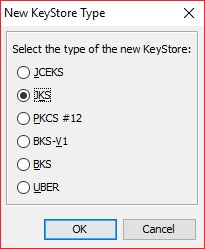
\includegraphics{../Dependancies/Keystore_Explorer/Type.jpg}
  \subsection{View and information}
You can view certificates and additional information with Keystore Explorer, view public and private key parts of certificates and other info such as subject alternative names by right clicking a certificate and choosing viable option from View option.
  \subsection{License}
Keystore Explorer is free to use utility, License is public.
  
\section{Generation and signing of certificates}

  \subsection{Keys, certificates and basic constraints}
  
    \subsubsection{Generate keys}
    
      \paragraph{Self-signed certificate}
It is possible to generate a key pair and self-signed certificate, simply click on icon or double click on blank space, choose algorithm and key length. Then you can choose all the other options such as Basic Constraints and Subject Alternative Name.

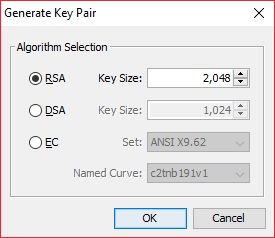
\includegraphics{../Dependancies/Keystore_Explorer/genKeys.jpg}
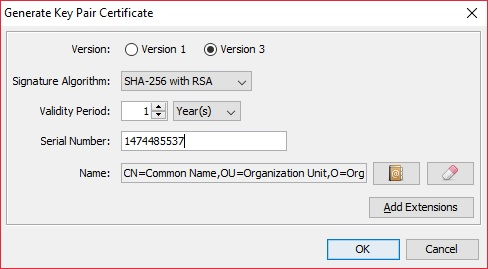
\includegraphics{../Dependancies/Keystore_Explorer/genCert.jpg}
You can also set up default pre-fill of Common Name, Organisational Unit, Organisation etc.

      \paragraph{Certificate Signing Request}
It is possible to make Certificate Signing Request in Keystore Explorer. Simply generate key pair certificate and then right click the generated certificate and choose Generate CSR option.
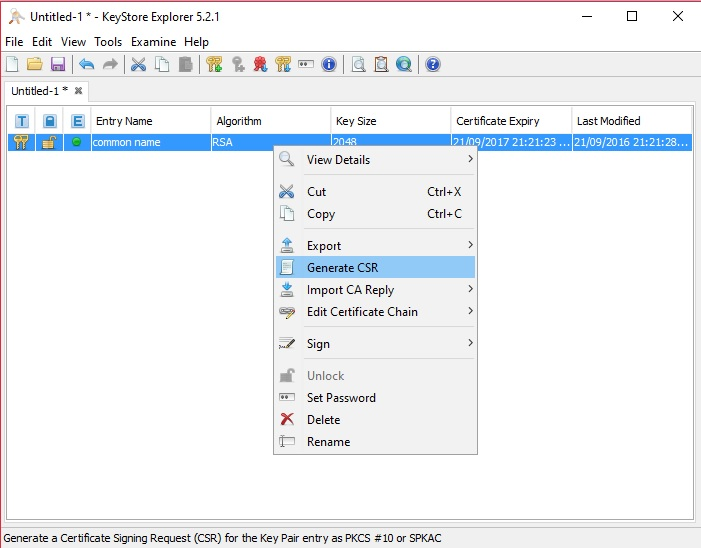
\includegraphics{../Dependancies/Keystore_Explorer/genCSR.jpg}
      \paragraph{Specify length}
Length is specified at the moment of key pair generation.
      \paragraph{Specify algorithm}
Algorithm of keys is specified when generating keys and the certificate hash function is chosen by certificate authority.
    \subsubsection{Basic constraints}

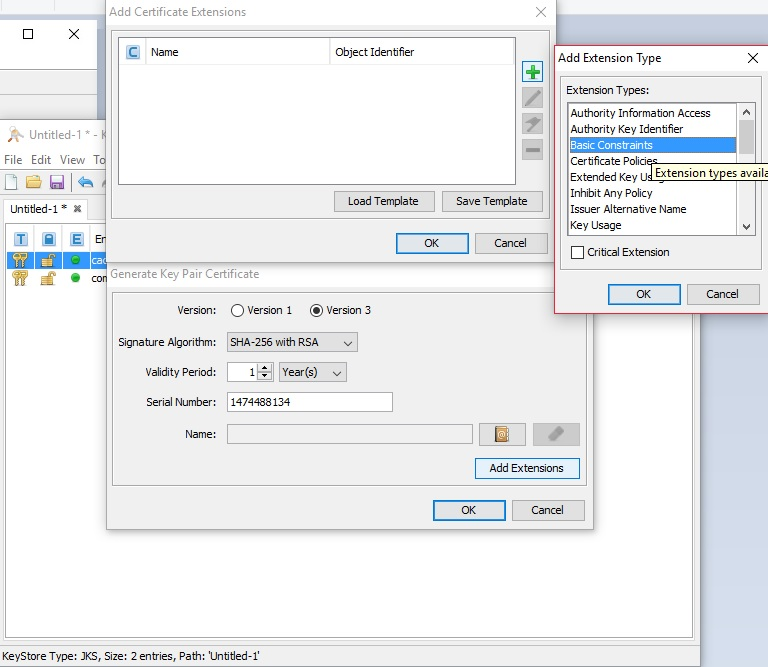
\includegraphics{../Dependancies/Keystore_Explorer/Basic_Constraints.jpg}

      \paragraph{Specify Type}
Specifying type is made while generating keys and certificate by changing v3 portion when asked during generation.
      \paragraph{Specify path length}
Specifying of max path length is made also by changing v3 part of x509 certificate during generation under Basic Constraints type.
  \subsection{Specifications}
  
    \subsubsection{Certificate Signing Request signing}
To sign a Certificate Signing Request simply right-click a Certificate Authority certificate and use the sign->CSR option. Then you need to import CA response that was generated in a desired place into a certificate from which the CSR was generated.

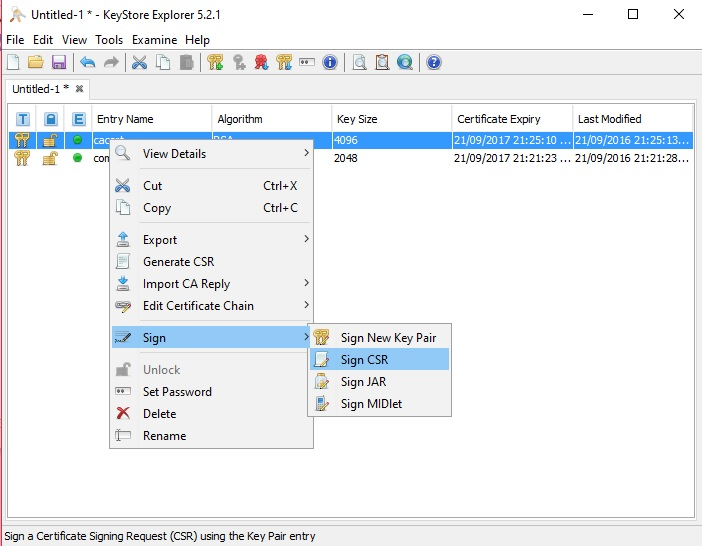
\includegraphics{../Dependancies/Keystore_Explorer/CSRsign.jpg}
    \subsubsection{Create combination of private key and signed chain}
To create combination of private key simply generate new key pair certificate, export private key part, import it back and then import to new certificate of private key a trusted chain.

    \subsubsection{Specify certificate validity}
Desired duration of certificate validity is asked during generation, but given whilst signing a Certificate Signing Request by Certificate Authority
    \subsubsection{Setting Subject Alternative Name for end certificates}
Setting of Subject Alternative Name for certificate is made during generation of certificate, under the add extentions option under the Subject Alternative Name part. Keystore Explorer allows to add both DNS and IP formats of SAN.
    \subsubsection{Support for Cryptographic Service Provider}
As Far as i know there is not support for using CSP.
\section{Conversions}

  \subsection{Exporting}
  
    \subsubsection{Certificate or certificate chain from a file}
It is possible to export a certificate or certificate chain from a keystore by simply right-clicking the chosen certificate and chosing export option.
    \subsubsection{Private key only}
It is possible to export a private key from a keystore by simply right-clicking the chosen certificate and chosing export->private key option.

  \subsection{Direct conversion between Java Keystore and PKCS\#12 file}
To change a type of file simply right-click on the blank space and choose change type option. In addition to changing a pkcs12 file type to JKS it is possible to change type of files between all supported types of Keystore Explorer.
  
  \subsection{Importing certificates and keys into storage files}
It is possible to import a certificate and/or key by chosing Import option.

%TEMPLATE FOR ALL OTHER TOOLS
\chapter{Tool Page Template}

\section{General}

  \subsection{Type}
  
  \subsection{View and information}
  
  \subsection{License}

  
\section{Generation and signing of certificates}

  \subsection{Keys, certificates and basic constraints}
  
    \subsubsection{Generate keys}
    
      \paragraph{Self-signed certificate}
      
      \paragraph{Certificate Signing Request}
      
      \paragraph{Specify length}
      
      \paragraph{Specify algorithm}
      
    \subsubsection{Basic constraints}
    
      \paragraph{Specify Type}
      
      \paragraph{Specify path length}
      
  \subsection{Specifications}
  
    \subsubsection{Certificate Signing Request signing}
    
    \subsubsection{Create combination of private key and signed chain}
    
    \subsubsection{Specify certificate validity}
    
    \subsubsection{Setting Subject Alternative Name for end certificates}
    
    \subsubsection{Support for Cryptographic Service Provider}
    
\section{Conversions}

  \subsection{Exporting}
  
    \subsubsection{Certificate or certificate chain from a file}
    
    \subsubsection{Private key only}
    
  \subsection{Direct conversion between Java Keystore and PKCS\#12 file}
  
  \subsection{Importing certificates and keys into storage files}
  


\end{document}
